\documentclass[../main.tex]{subfiles}

\begin{document}
\section{Contexto}
En 1947, Alan Turing en su conferencia ante la London Mathematical Society \cite{Turing1947} aportaba su visión a la vieja pregunta: ¿pueden pensar las máquinas? y proponía el famoso Test de Turing, objeto de inmensa influencia y debate en el campo de la Inteligencia Artificial. Mucho ha transcurrido desde entonces, con el debate sobre la capacidad de las máquinas transcendiendo los límites del mundo académico para impregnar el imaginario colectivo, con películas como Terminator (1984).
\begin{figure}[h!]
    \centering
    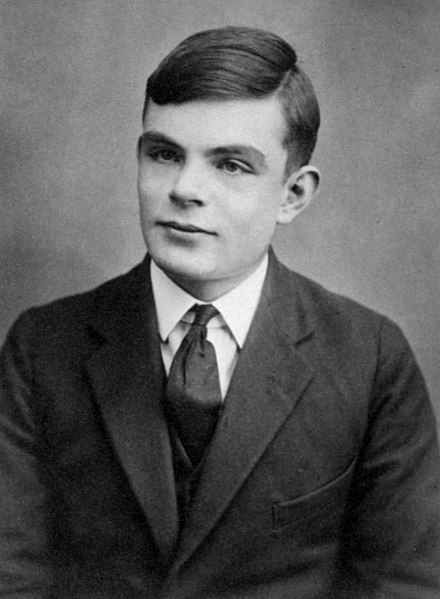
\includegraphics[width=0.25\textwidth]{imagenes/Alan_Turing_Aged_16.jpg}
    \caption[Alan Turing con 16 años]{Alan Turing con 16 años. Imagen obtenida de \cite{Desconocido1928}.}
    \label{fig:alan_turing_16}
\end{figure}

Por otra parte, una de las formas de creatividad humana por excelencia es la pintura. Una de sus corrientes, el Impresionismo, buscaba reaccionar contra la pintura convencional plasmando sensaciones y la fugacidad del instante \cite{EditorialSalvat2006}.

\begin{figure}[h!]
    \centering
    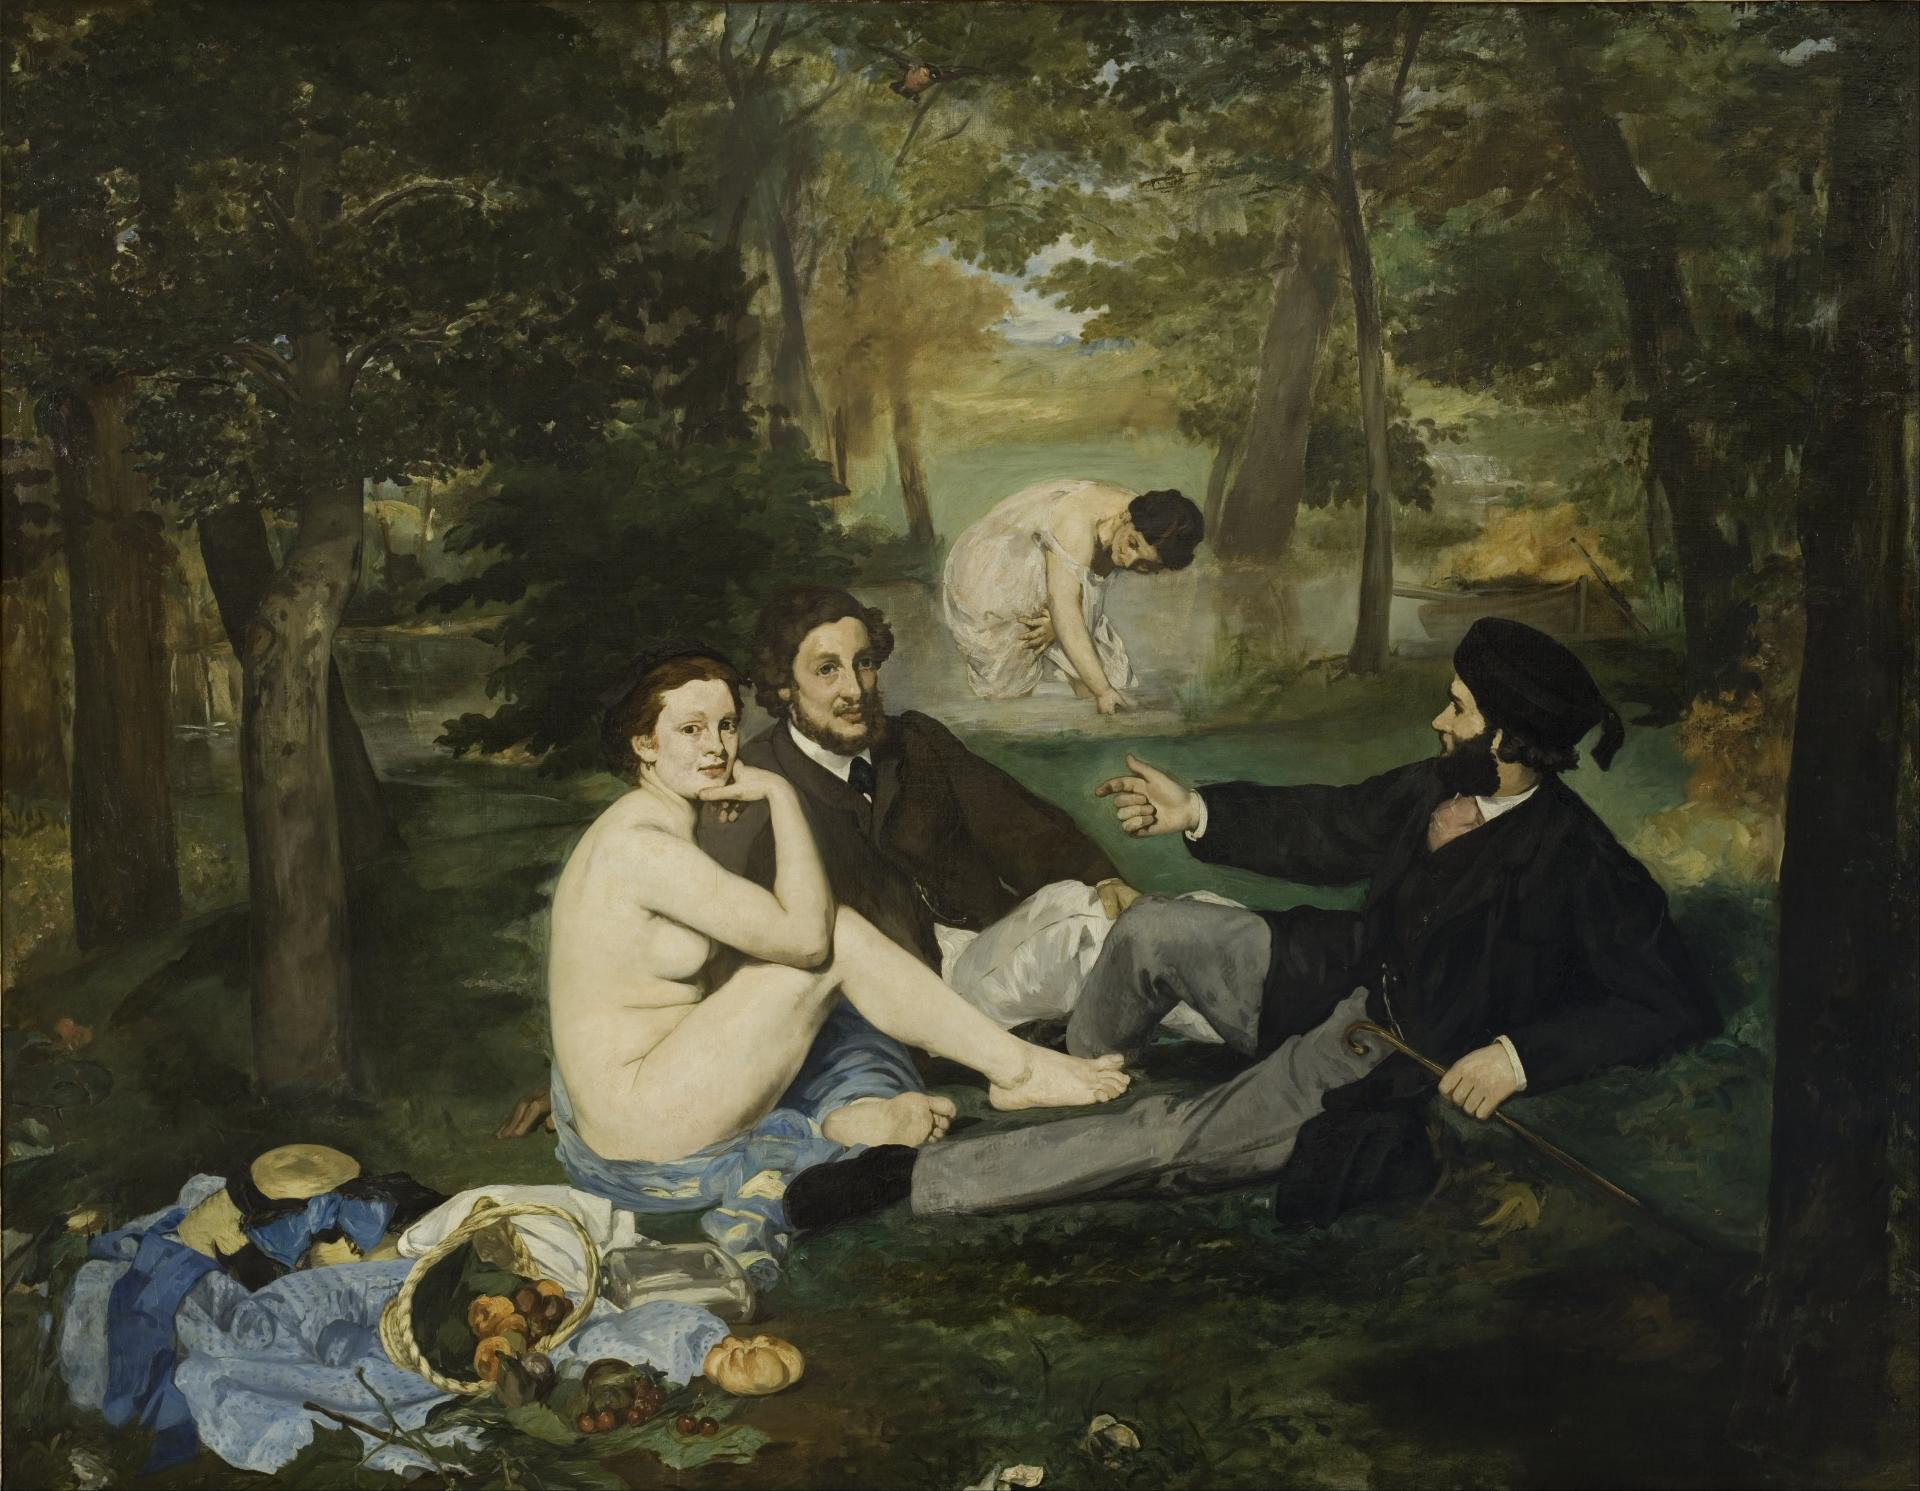
\includegraphics[width=0.5\textwidth]{imagenes/Almuerzo sobre la hierba.jpg}
    \caption[Almuerzo sobre la hierba, de Édouard Manet]{Almuerzo sobre la hierba, de Édouard Manet (Musée d'Orsay, Paris). Extraído de \cite{Manet1863}.}.
    \label{fig:manet_almuerzo_hierba}
\end{figure}

\newpage
Asimismo, el Impresionismo fue un movimiento muy influyente en su apogeo (segunda mitad del siglo XIX) debido a que es el punto de unión entre dos fenómenos: la captación de la realidad por el artista mediante la pintura, iniciada en los albores del siglo XV; y la genésis del Arte Contemporáneo, en la que las \textit{emociones} adquieren más peso en la técnica del artista, por lo que no cabe duda que fue un movimiento extremadamente creativo.
\newline

De vuelta al siglo XXI, en el mundo de la Inteligencia Artificial se han producido enormes avances en los últimos años: tenemos máquinas que pueden vencer a jugadores profesionales en juegos de gran tradición y prestigio como Go (AlphaGo versus Lee Sedol) \cite{Metz2016}, avanzados sistemas de reconocimiento facial implantados masivamente (Proyecto Skynet) \cite{Diez2019}, investigaciones sobre la telemedicina y el telediagnostico en nuestra propia escuela \cite{Aldana2019} entre otros muchos, lo que ha originado una auténtica tormenta de controversia sobre las capacidades de la Inteligencia Artificial y de sus implicaciones éticas y morales.
\newline

Todo esto da pie a plantearse la pregunta: ¿puede crear arte una máquina? \cite{Garcia2017} \cite{Serradilla2017}, y de ser así ¿podría realizar algo tan creativo como cuadros impresionistas?
\section{Objetivos}
El objetivo principal de este Trabajo de Fin de Grado consiste en la obtención e implantación de un modelo de Inteligencia Artificial para la emulación \"razonable\" de los pintores impresionistas Monet, Van Gogh y Cézanne, de ser posible con el estado del arte actual. La implementación de dicho modelo suministrará una imagen de entrada, es decir, no se busca que suministre un cuadro aleatorio, sino un cuadro \textit{inspirado} en una imagen ya existente, emulando a la pintura al aire libre característica del Impresionismo.
\subsection{Objetivos secundarios}
Además del objetivo principal, se han especificado los siguientes objetivos secundarios:
\begin{enumerate}
    \item Realizar una reflexión sobre la capacidad actual de la Inteligencia Artificial respecto a la emulación de la creatividad propia de las Bellas Artes.
    \item Aprender el lenguaje de programación Python y las plafaformas Keras y Tensorflow.
    \item Construir una arquitectura software que permita la incorporación de otros pintores de forma sencilla para el lector.
    \item Explorar las posibilidades de la nube para el desarrollo de modelos de Inteligencia Artificial.
    \item Elaborar una API REST para la implementación de servicios web para expandir las posibilidades del modelo construido previamente.
    \item Aprender \LaTeX{} para la realización del presente documento.
\end{enumerate}

\section{Estructura del documento}
Tras esta introducción, el resto de este documento se estructura en los siguientes apartados:
\begin{itemize}
    \item \textbf{Estado del arte}: Se expone el Impresionismo pictórico como corriente artística, junto a las características de los tres pintores que trataremos de emular mediante el modelo de Inteligencia Artificial. Por otra parte, se exponen los conceptos de Inteligencia Artificial, Machine Learning y Redes Neuronales, los diversos tipos de redes neuronales relacionados con la Visión Artificial y por último las Redes Generativas Adversativas Cíclicas, que es la solución propuesta para realizar este Trabajo de FIn de Grado
    \item \textbf{Tecnologías utilizadas}: En esta sección se exponen las tecnologías utilizadas para el desarrollo del proyecto de forma significativa, con la finalidad de que el lector comprenda qué son y por qué se han usado tales herramientas en la elaboración del proyecto.
    \item \textbf{Desarrollo del proyecto}: Este capítulo conforma el núcleo del presente documento: se aborda el diseño del sistema, los datos utilizados para entrenar el modelo, la documentación del sistema para que el lector pueda replicar el proyecto y realizar modelos propios y los resultados obtenidos.
    \item \textbf{Conclusiones}: Se desarrollan las conclusiones obtenidas de la investigación y del desarrollo del proyecto, además de la experiencia personal del autor en la realización del mismo.
    \item \textbf{Impacto social}: Este apartado contiene una reflexión sobre el impacto social y medioambiental de este Trabajo Fin de Grado.
    \item \textbf{Lineas futuras}: En esta sección se detallarán las posibles ampliaciones y mejoras del proyecto a juicio del autor. 
    \item \textbf{Anexos}: En los Anexos se detallan los entornos de desarrollo utilizados en la elaboración del proyecto, así como el código fuente del mismo.
\end{itemize}

\end{document}